\section{Boundary conditions}\label{sec:lbm:bound}
In all physical situations, when solving a differential equations on a
domain, conditions for what is happening on the boundary of the domain
must be specified. So far, only the update rule for $\fii$ on the
interior of this domain has been treated. In this section we will
also define rules for the boundaries of the domain. The nodes in the
interior and the boundary will be referred to as \emph{interior nodes}
and \emph{boundary nodes} respectively. Typically, a boundary
condition in a macroscopic variable, e.g. velocity, is specified from
the physical problem. This condition must be translated into a
condition for the distribution function, $\fii$, on the statistical
level. In this section some, to this work, useful boundary conditions
will be formulated and discussed.

\begin{figure}
\begin{center}
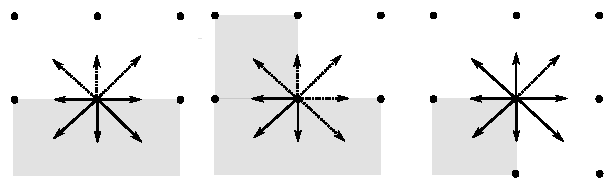
\includegraphics[width=0.9\textwidth]{fig/bb.pdf}
\end{center}
\caption[Three different boundary situations in the LBM.]{Three
  distinct boundary situations that in general has to be treated
  differently. From left to right, a straight boundary, a corner and
  an edge. Grey areas are outer of the domain. The solid arrows
  corresponds to known directions of the distribution function and
  dotted lines to unknown.}
\label{fig:lbm:bounds}
\end{figure}

\subsection{Bounce-back boundaries}\label{sec:lbm:bb}
The lattice-Boltzmann approach is often praised for its rather
straight-forward easiness of implementing boundary conditions. One of
the simplest and most commonly used is the bounce-back rule. It is a
mesoscopic rule for implying a Dirichlet condition on the first
moment. In the case of specifying boundary conditions for
Navier-Stokes, it may be used to set a velocity at a boundary,
typically at wall boundaries the velocity is set to zero.

The bounce-back rule for setting the first moment to zero reads

\begin{equation}
\fii^{(bb)} = f_{i^*}
\end{equation}
where $\mathbf{c}_{i^*}$ is the direction opposite to $\ci$. This
justifies the name of the rule, all pseudo particles are propagated in
a direction opposite to where they came from, i.e. bounced back. If
the boundary nodes are updated between the collision and streaming
step, all directions should be updated with its opposite
counterpart. However, if the update is performed after the streaming
step, only the unknown directions are to be updated, see
fig. \ref{fig:lbm:bounds}. These two schemes are referred to full-way
and half-way bounce-back. If a non-zero Dirichlet condition is
desired, it is possible to add some momentum to suitable directions.

It is possible to show that, in the case of a straight boundary, the
actual boundary is with second order accuracy located half a node-node
distance into the computational domain \cite{junk-boundary}. Thus, the
boundary will not be located at the boundary node. 

As suggested earlier in this section, this type of local boundary
conditions allows for easy implementation of more or less arbitrary
boundaries. In fig. \ref{fig:lbm:cool_flow}, an example of 2D flow in a
complicated domain is shown. At the walls in the figure, bounce-back
conditions are used.

\begin{figure}
\begin{center}
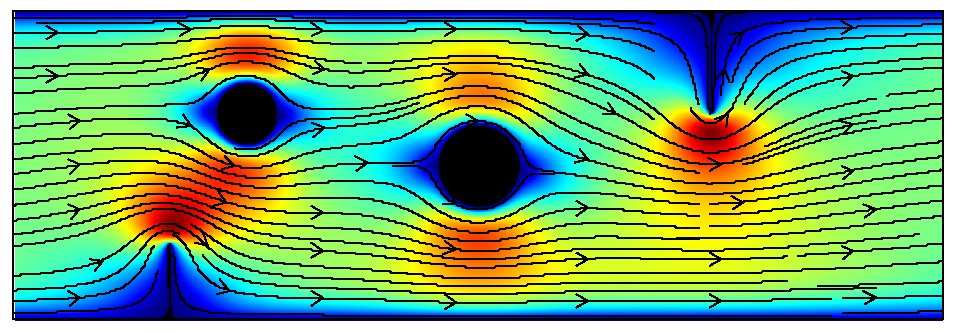
\includegraphics[width=0.9\textwidth]{fig/comp_bound_u.pdf}
\end{center}
\caption[Example of flow in a non-trivial geometry.]{Example of flow
  in a non-trivial geometry where bounce-back boundaries are used.}
\label{fig:lbm:cool_flow}
\end{figure}

\subsection{Slip boundaries}\label{sec:lbm:mirror}
A zero friction (slip) boundary condition may be imposed by the
following rule for the straight boundary situation in
fig. \ref{fig:lbm:bounds}. Instead of making all pseudo particles
``bounce back'', they are reflected in a mirror-like manner, see
fig. \ref{fig:lbm:slip}. This gives that the component normal to the
boundary of the first moment is zero while the tangential component is
unchanged. In this work, this condition is used to set the
ion flux through the boundary to zero, eq. \eqref{eq:et:j0}.

It is not as straight-forward to define rules at corner and edge
nodes, as for the straight boundary nodes. From tests, it has been
shown that adequate accuracy may be obtained by treating the corner or
edge as two perpendicular straight boundaries and mirror reflect half
of the distributions at each plane respectively. 

\begin{figure}
  \centering
  \subfloat[Bounce-back
    ]{\label{fig:lbm:no_slip}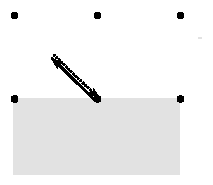
\includegraphics[width=0.35\textwidth]{fig/no_slip.pdf}}      
  \hspace{5pt} \subfloat[Mirror reflection
  ]{\label{fig:lbm:slip}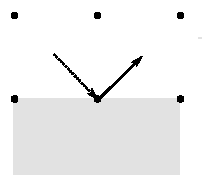
\includegraphics[width=0.35\textwidth]{fig/slip.pdf}}
  \caption[Intuitive scheme for the bounce-back and mirror reflection
    conditions.]{Intuitive scheme for an incoming pseudo particle for
    two common boundary conditions in the LBM. The bounce-back rule
    (a) and mirror reflection (b).}
  \label{fig:lbm:bbs}
\end{figure}

\subsubsection{With momentum addition}\label{sec:lbm:mod_mirror}
In the case with the fixed surface charge boundary condition,
eq. \eqref{eq:et:fix_c}, we do not wish to set the normal component to
zero but to some value of the surface charge. This is realised by
adding some ``momentum'' in the three directions pointing in to the
domain. The total surface charge may be divided between the directions
in different proportions, in this work it is however evenly
distributed, i.e. one third per direction. 

%\subsection{he-zou, constant density/velocity}\label{sec:lbm:hezou}

%\subsection{Maybe something on non-local boundary conditions}
